\section{Mechanical Analysis}
\label{sec:analysis}
In the following paragraphs the effects of the impact of the car on the femur of
the pedestrian are investigated. First an estimation of the forces exerted on
the femur is made. Then a force diagram and torque diagrams are calculated.
Based on these diagrams the stresses in the bone are estimated and by comparing
the stresses with experimental data of previous research the probability that
the bone will fail is estimated.

\subsection{Calculating impact force}
We start from the conservation of momentum law in the direction the car is
traveling. This assumes a perfect ellastic collision, which is a very
crude approximation of reality. Because the velocity of the pedestrian in this
direction is zero, so is his momentum. \autoref{fig:events} shows that the car
and the pedestrian cling together during the first few seconds after time of impact, so
we consider them as one system with one momentum.
\begin{equation}
	p_{C_0} + 0 = p_1
\end{equation}

% \begin{equation}
% 	\frac{m_C \cdot v_{C_0}^2}{2} + \frac{m_P \cdot v_{P_0}^2}{2}  = 
% 	\frac{m_C \cdot v_{C_1}^2}{2} + \frac{m_P \cdot v_{P_1}^2}{2}
% \end{equation}

\begin{equation}
	m_C \cdot v_{C_0} + 0 = (m_C + m_P) \cdot v_1
\end{equation}

Solve for $v_1$.
\begin{equation}
	v_1 = \frac{m_C}{m_C + m_P} \cdot v_{C_0} 
	= \frac{2400\text{ kg}}{2480\text{ kg}} \cdot 10 \text{ m/s}
	\approx 9.68 \text{ m/s}
\end{equation}

From this, we can calculate the force acting on the pedestrian.
\begin{equation}
	F' = \frac{\Delta p}{\Delta t}
\end{equation}

The equation shows that the force $F$ is also dependent on the time interval
$\Delta t$ in which the collision occurs. When two hard materials hit each
other, e.g. a club hitting a golfbal, this interval is approximately $400 \mu
s$\footnote{http://www.golfswing.com.au/139}. On the other hand, the typical
impact time - from full speed to standstill - of a car crashing into a wall is
about 100ms \cite{crash_mech}
\footnote{http://auto.howstuffworks.com/car-driving-safety/accidents-hazardous-conditions/crash-test.htm}.
This interval is larger because of crumple zones. However, because our car is
equipped with a bullbar, and because we only take into account the initial
event, we estimate $\Delta t \approx 10$ms.

Plugging this value into the equation gives:
\begin{equation}
	F' = \frac{80\text{ kg} \cdot 9.68\text{ m/s}}{0.01\text{ s}} = 77440\text{ N}
\end{equation}

We assumed a soft tissue damping factor of roughly 15\%, which allows us to
calculate the resulting foce on the femur:
\begin{equation}
	F = 0.85F' = 65824\text{ N}
\end{equation}

\subsection{Discussion on force and torque diagrams} 
%TODO we have a chapter devoted to assumptions, do we need to bring it up here again?

In \autoref{fig:hyper1} the complex system of the leg of the pedestrian getting
hit by the bull bar of the car is visualised. In order to make a mechanical
analysis of this system a number of assumptions had to be made. To make the
assumptions three things were taken into consideration. First,
\cite{snedeker2005assessing} proposed a set of boundary conditions to analyse
the impact of a car bumper on the leg of a pedestrian. In this paper it is
suggested to assume the pelvis to be �fixed� -- such that the pelvis has a
horizontal velocity of zero -- during the first moments of the crash. Second, we
analysed the deformation of a set of mechanical systems and compared these with
our visual analysis of the legs of dummies in crash
tests\footnote{\url{https://www.youtube.com/watch?v=tNRHB75NiIc}}. The main
parts in all mechanical systems were the pelvis (suggestions: clamped, simply
supported or hinge), the femur (suggestion:
a beam), the knee (suggestions: hinge, simple supported or simply a
uninterrupted beam which represents femur, knee and bones in lower leg), the
bones in the lower leg (a beam) and the foot and ankle (suggestions: clamped,
simply supported or hinge). For all combination of the mechanical
representations of these main mechanical parts the line of deformation was
drawn. Finally, the system represented in \autoref{fig:hyper1} was chosen.

%TODO check scharnieren in figuren

 \begin{figure}[htp]
\begin{center}
  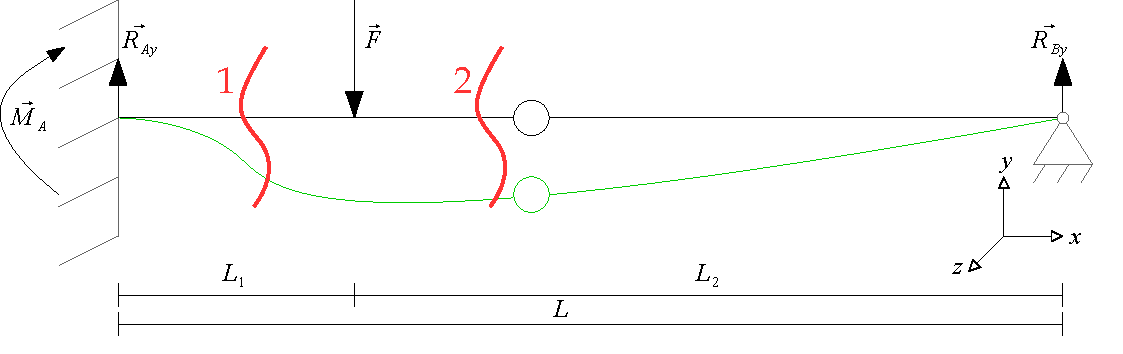
\includegraphics[page=1,width=\textwidth]{img/hyper.pdf}
  \caption{Schematic of the system under consideration. The pelvis (left) is
  modeled as a clamp, while the angle (right) is replaced by a hinge. The knee
  (circle) is merely added for visual guidance, it does not play any
  significant part in this analysis. The total length $L$ is split up in $L_1$
  and $L_2$ at the point of impact.}
  \label{fig:hyper1}
\end{center}
\end{figure}

After the mechanical system was decided upon, the force and torque equilibrium
equations were calculated. 

\begin{equation}
	\Sigma F=0: R_{Ay} + R_{By} - F = 0
\end{equation}

\begin{equation}
	\Sigma M_B=0: L_2 F - (L_1 + L_2)R_{Ay} - M_A = 0 
\end{equation}

From these equations it is clear we have a hyperstatic sytem of level 1, which
means we have three unknowns and only two equations. Therefore, this system has
to be solved using �the method of the chord�. The first step in applying this
technique is choosing two points $a$ and $b$ that are fixed in your system. Then
a point $c$ is determined which is situated between point $a$ and $b$ and for
which you want to calculate the deformation in the system due to external forces
and torques. In this case point $c$ coincides with point $a$. Next the torque %
%TODO Torque or bending moment
diagram $M$, taking into account all external forces, is calculated. From this
torque diagram $M$ the reduced torque $M_{red}$ is deduced by dividing M by the
multiplication of the Young�s modulus and the moment of inertia of the system
($EI$). In this way the stiffness of the system is also taken into account which
will allow us to get an exact solution for the hyperstatic mechanical system.
After this the reduced torque diagram is treated as a distributed force acting
on the entire length of the beams. To calculate the equivalent forces of these
distributed forces the reduced torque diagram is divided into triangular parts
of which an $F_{eq}$ is calculated each time. Then the reaction force in point
$c$ is determined. The method of the chord assumes the reaction force in this
point to be the same as the angle of deformation in that point.

In order to solve the hyperstatic system it has to be divided into two
subsystems: a main system (\autoref{fig:hyper2main}) and a recovery system
(\autoref{fig:hyper3recovery}). The main system is the hyperstatic system made
static again by cancelling one force or torque. In this case we chose to cancel
the torque of the clamped pelvis. The task of the recovery system is to restore
the distorted line of deformation of the main system to the line of deformation
of the initial hyperstatic system. Therefore, a torque $m_a$ is added in the
recovery system. The method of the chord is applied on both systems and then the
results of the two systems are superimposed to obtain the results for the
initial hyperstatic system.

 \begin{figure}[htp]
\begin{center}
  \includegraphics[page=2,width=\textwidth]{img/hyper.pdf}
  \caption{The main system (HS).}
  \label{fig:hyper2main}
\end{center}
\end{figure}

\begin{figure}[htp]
\begin{center}
  \includegraphics[page=3,width=\textwidth]{img/hyper.pdf}
  \caption{The recovery system (hs).}
  \label{fig:hyper3recovery}
\end{center}
\end{figure}

\subsubsection{Analysis of the main system}
First, we calculate $R_A$ (and thus $\theta_{HS}$) in \autoref{fig:hyper4}.
\begin{equation}
	M_b = M(L_1) = R_A \cdot L_1 = \frac{-L_1 \cdot L_2}{L_1 + L_2} \cdot F
\end{equation}

\begin{equation}
	M_{b,red} = \frac{-L_1 \cdot L_2}{L_1 + L_2} \cdot \frac{F}{EI}
\end{equation}

\begin{equation}
	\Sigma M=0: \frac{2}{3} L_2 F_{e_2} + (L_2 + \frac{1}{3}L_1) F_{e_1} - R_A (L_1
	+ L_2) = 0
\end{equation}

Solve for $R_A$:
\begin{equation}\label{eq:RA}
	R_A = \frac{\frac{2}{3} L_2 F_{e_2} + L_2 F_{e_1} + \frac{1}{3}L_1 F_{e_1}}{L_1 +
	L_2} = \theta_{HS}
\end{equation}

We also know $F_{e_1}$ and $F_{e_2}$: 
\begin{equation}
	F_{e_1} = \frac{-L_1 L_2}{L_1+ L_2} \frac{F}{EI} \frac{L_1}{2}
\end{equation}

\begin{equation}
	F_{e_2} = \frac{-L_1 L_2}{L_1+ L_2} \frac{F}{EI} \frac{L_2}{2}
\end{equation}

Plugging these equations in \autoref{eq:RA} gives:
\begin{equation}
	R_A = \frac{-1}{3} \frac{L_1 L_2^3 F}{(L_1 + L_2)^2 EI} - \frac{L_1^2 L_2^2
	F}{(L_1 + L_2)^2 2EI} - \frac{-1}{6} \frac{L_1^3 L_2 F}{(L_1 + L_2)^2 EI} =
	\theta_{HS}
\end{equation}

\begin{figure}[htp]
\begin{center}
  \includegraphics[page=4,width=\textwidth]{img/hyper.pdf}
  \caption{Reduced torque diagram $M_{red}$ of the main system.}
  \label{fig:hyper4}
\end{center}
\end{figure}

\subsubsection{Analysis of the recovery system}
We repeat this exercise for the recovery system in \autoref{fig:hyper5}.
\begin{equation}
	M_b = -m = -m_a
\end{equation}

\begin{equation}
	M_{b,red} = \frac{-m}{EI}
\end{equation}

\begin{equation}
	\Sigma M_b = 0: \frac{2}{3}(L_1 + L_2)F_e - (L_1+L_2) R_a = 0 
\end{equation}

Solve for $R_a$:
\begin{equation}
	R_a = \frac{\frac{2}{3}(L_1 + L_2)F_e}{L_1 + L_2} = \frac{2}{3} F_e
\end{equation}

We also know $F_e$:
\begin{equation}
	F_e = \frac{-m}{EI} \frac{L_1 + L_2}{2}
\end{equation}

So we can rewrite $R_a$ as:
\begin{equation}
	R_a = \frac{-2}{3} \frac{m}{EI} \frac{L_1 + L_2}{2} = \theta_{hs}
\end{equation}

\begin{figure}[htp]
\begin{center}
  \includegraphics[page=5,width=\textwidth]{img/hyper.pdf}
  \caption{Reduced torque diagram of the recovery system.}
  \label{fig:hyper5}
\end{center}
\end{figure}

\subsubsection{Combining both systems}
To combine the two systems, the following equation must hold:
\begin{equation}
	\theta_{HS} + \theta_{hs} = 0
\end{equation}

\begin{equation} %TODO 1/3 aangeven?
	\frac{-1}{3} \frac{L_1 L_2^3 F}{(L_1 + L_2)^2 EI} - \frac{L_1^2 L_2^2
	F}{(L_1 + L_2)^2 2EI} - \frac{1}{6} \frac{L_1^3 L_2 F}{(L_1 + L_2)^2 EI} -
	\frac{2}{3} \frac{m}{EI} \frac{L_1 + L_2}{2} = 0
\end{equation}

Solve for m:
\begin{equation}
	m = \frac{-2 L_1 L_2^3F - 3 L_1^2 L_2^2 - L_1^3 L_2 F}{2(L_1 + L_2)^3}
\end{equation}

Using $L_1 = 0.154$m, $L_2 = 0.8$m and $F = 65824$N, we can calculate $M_A$:
\begin{equation}
	M_A = -m = 7814.44\text{Nm} %TODO dus M_A == M_b ???
\end{equation}

\subsubsection{Solving the original system}
With this knowledge, we can finally solve the original system and construct the
accompanying force (\autoref{fig:hyper6}) and torque (\autoref{fig:hyper7})
diagrams.

%TODO waarom mocht dit ook alweer?
\begin{equation}
	R_{Ay} = \frac{L_2}{L_1 + L_2} F = 55 198.32
\end{equation}

\begin{equation}
	R_{By} = \frac{L_1}{L_1 + L_2} F = 10 625.68
\end{equation}

\begin{equation} %TODO M what?
	 M = \frac{L_1 L_2}{L_1 + L_2} F = 8 500.54
\end{equation}

\begin{equation} %TODO M what?
	 M = \frac{L_2 M_A}{L_1 + L_2} = 6 552.98
\end{equation}

\begin{figure}[htp]
\begin{center}
  \includegraphics[page=6,width=\textwidth]{img/hyper.pdf}
  \caption{Force diagram of the original system.}
  \label{fig:hyper6}
\end{center}
\end{figure}

\begin{figure}[htp]
\begin{center}
  \includegraphics[page=7,width=\textwidth]{img/hyper.pdf}
  \caption{Torque diagram of the original system.}
  \label{fig:hyper7}
\end{center}
\end{figure}

The forces applied on the upper part of the upper leg are definitely the
largest: they are five times larger than the forces applied on the lower parts.
Nevertheless, both distributed forces are of significant magnitude: 55,2 kN  and
10,6 kN. As they are exerted in the transverse direction on the femur, it is
very likely they will cause a fracture of the bone. All long bones have
anisotropic structure characteristics. This causes them to be stronger in the
longitudinal direction than in the transverse direction. The femur is one of the
strongest bones in the body and is able to carry loads up to thirty times the
body weight. (VERSCHILLENDE KEREN GELEZEN MAAR VINDT REF NIET MEER ) In our
case this means the femur can withstand a load of 23 544 N in the longitudinal
direction. %TODO but what with the transverse direction?

The torques due to the applied forces are also of significant magnitude and will
therefore cause the bone to bend. Not surprisingly, very soon the bone will
fracture under these loading conditions.

\subsection{Calculating stress in the femur}
In this section, we calculate the stress $\sigma$ in the femur, assuming it
has not yet broken. For this, we need the applied force $F$ and the contact area
$A$. We already know $F$, so this section will focus on estimating $A$. To do
so, we make use of Hertz theory. We model both the femur and the bull bar as
cylinders, and assume they are in direct contact. This theory requires three
main assumptions to hold true:
\begin{enumerate}
  \item both materials must have a similar Young's modulus
  \item both surfaces must deform
  \item the contact area must be relatively small compared to the two bodies in
  contact
\end{enumerate}

The first assumption will not hold in the case of a stainless steel bull bar,
but it can work for an aluminium bull bar.

Out goal is to calculate the area $A$ of the circular contact area. This
requires a contact radius $a$:
\begin{equation}
	a = \sqrt{Rd}
\end{equation}

We estimate the radius of the femur and bull bar as respectively $R_{bone} =
12.15$mm and $R_{bar} = 30.00$mm. The diameters $D_{bone}$ and $D_{bar}$ are
obviously double those values. Combining these two radii with the
formule below yields $R$:
\begin{equation}
	\frac{1}{R} = \frac{1}{R_{bone}} + \frac{1}{R_{bar}} = 115.3 \text{1/m} \Leftrightarrow R = 0.0087\text{m} 
\end{equation}

We can also calculate $d$ -- the total elastic compression at the contact
surface, measured along the line of the applied force $F$ -- using a formule
proposed by \cite{puttock1969elastic}:
%TODO nu or v?
\begin{equation}
	d = \frac{(3\pi)^\frac{2}{3}}{2} \cdot F^\frac{2}{3} \cdot (\nu_{bone} +
	\nu_{bar})^\frac{2}{3} \cdot \left(\frac{1}{D_{bone}}\right)^\frac{1}{3}
\end{equation}

%TODO dimensions?
Herein, $\nu_{bone}$ and $\nu_{bar}$ are given by:
\begin{equation}
	\nu_{bone} = \frac{1 - \nu_{femur}^2}{\pi E_{femur}} = \frac{1 - 0,37^2}{\pi \cdot 20\text{ GPa}} = 1,3737 \cdot 10^{-11}
\end{equation}
\begin{equation}
	\nu_{bar} = \frac{1 - \nu_{Al}^2}{\pi E_{Al}} = \frac{1 - 0.32^2}{\pi \cdot 69\text{ GPa}} = 4.1408 \cdot 10^{-12}
\end{equation}

Plug in all known variables, and we get this result: %TODO dimensions?
\begin{equation}
	d = \frac{(3\pi)^\frac{2}{3}}{2} \cdot (65824\text{ N})^\frac{2}{3} \cdot (1,3737 \cdot 10^{-11} +
	4.1408 \cdot 10^{-12})^\frac{2}{3} \cdot \left(\frac{1}{0.0243\text{ m}}\right)^\frac{1}{3} = 0.0008585\text{ m}
\end{equation}

At last, we can find $A$ and thus $\sigma$:
\begin{equation}
	A = \pi  a^2 = \pi R d = 0.000023465 \text{ m}^2
\end{equation}

\begin{equation}
	\sigma = \frac{F}{A} = \frac{65824\text{ N}}{0.000023465 \text{ m}^2} = 2 805 2 \cdot 10^5\text{ Pa} \approx 2.8\text{ GPa}
\end{equation}

%TODO G=?
%Poisson ratio:
%\begin{equation}
%	\nu = \frac{E}{2G - 1}
%\end{equation}


\subsection{Will the femur break?}
Compare to the table in \autoref{fig:femurprop}: transverse compression
of max 133 MPa for femur.

Calculated transverse stress: 3.3 GPa
Femural bone will fail!

%TODO: F is linear in speed. Reaction forces and torques are linear in F.
% -> easy to calculate maximum speed so that femur won't break? 

\begin{figure}[htp]
\begin{center}
  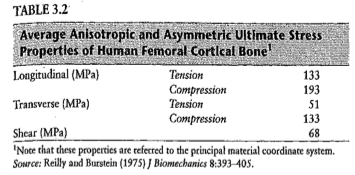
\includegraphics{img/properties_femur.png}
  \caption{Properties of the femur. \cite{Ob}}
  \label{fig:femurprop}
\end{center}
\end{figure}
